\documentclass[12pt]{amsart}
\pagestyle{plain}

\usepackage{amsthm, setspace, framed, hyperref}
\usepackage[pdftex]{graphicx}
\usepackage{enumerate}

\usepackage[left=1in, right=1in, top=1in, bottom=1in]{geometry}
\setlength\parindent{0pt}

\theoremstyle{plain}
\newtheorem{thm}{Theorem}[section]
\newtheorem{lem}[thm]{Lemma}
\newtheorem*{cor}{Corollary}
\newtheorem{quest}{Question}
\theoremstyle{definition}
\newtheorem*{defn}{Definition}
\newtheorem*{ex}{Example}

\begin{document}
\title[]{Cryptography Mission 02 Dossier}
\begin{tabular*}{\textwidth}{@{\extracolsep{\fill}}l l}
MATH/CSCI 408  & Name: \rule{7cm}{0.5pt} \\
\hline\hline
\end{tabular*} \\
\maketitle

\begin{center}\textbf{Deadline: Thursday, 31 August 2017 at 10:50am}\\

This mission covers Sections 2.1, 2.2, and 2.3.
\end{center}

\begin{framed}
Check one:\\

\framebox(12,12){} I received help from the following classmate(s) on this assignment:\\

\rule{15cm}{0.5pt}.\\

\framebox(12,12){} I did not receive any help on this assignment.
\end{framed}


\section{Graded Problems}

\begin{enumerate}[1.]
	\item (T\&W 2.13 \# 4)  Consider an affine cipher ($\bmod 26$).  You do a chosen plaintext attack using \texttt{hahaha}.  The ciphertext is \texttt{NONONO}.  Determine the encryption function.\\ \begin{framed}\vspace{2in}\end{framed}
	 \newpage  \item This problem involves the Dancing Men code from a Sherlock Holmes story.
		\begin{center}
			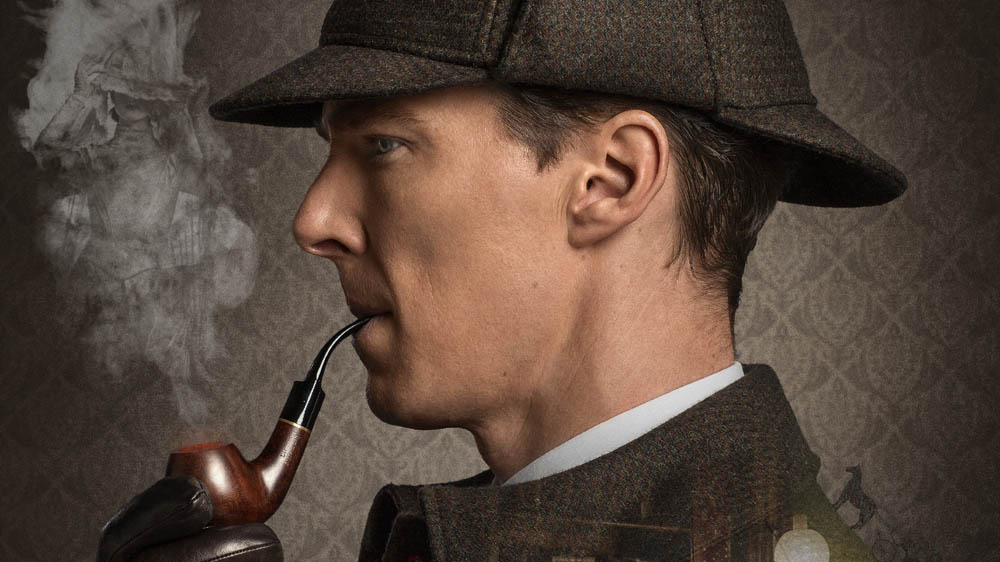
\includegraphics[height=1in]{Sherlock.jpg}\\
			\tiny{(Image from \url{http://www.cultbox.co.uk/reviews/episodes/sherlock-2016-special-review-the-abominable-bride}.)}
		\end{center}
		
		\begin{enumerate}[a.]
			\item Read Section 2.5 (Sherlock Holmes), and describe (in a paragraph) how Sherlock figures out which dancing man represents the letter \texttt{e} as well as the letter \texttt{r}.\\ \begin{framed}\vspace{2in}\end{framed}
			\item Explain in one sentence what the little flags mean.\\\begin{framed}\vspace{1in}\end{framed}
			\item Draw the dancing men figures that would correspond to the plaintext: \texttt{math}.\\ \begin{framed}\vspace{1.5in}\end{framed}
		\end{enumerate}
		 \newpage \item (T\&W 2.14 \# 2)  The following ciphertext was the output of a shift cipher:
		\begin{center}
			\texttt{LCLLEWLJAZLNNZMVYIYLHRMHZA}
		\end{center}
		By performing a frequency count, guess the key used in the cipher.  What is the decrypted plaintext?\\ \begin{framed}\vspace{2in}\end{framed}
				
	\item Read the Wikipedia article on the Pigpen cipher:\\ \url{https://en.wikipedia.org/wiki/Pigpen_cipher}.
	\begin{enumerate}[a.]
	\item Replicate the set of all graphical symbols on your homework here:
	\begin{framed}
	\vspace{1.8in}
	\end{framed}
	\item Encrypt the message ``you only live twice" using the Pigpen cipher.
	\begin{framed}
	\vspace{2in}
	\end{framed}
	\end{enumerate}
\end{enumerate}

\section{Honors Section Problem}
 (T\&W 2.13 \# 6) Suppose you encrypt using an affine cipher, then encrypt the encryption using another affine cipher (both are working $\bmod 26$).  Is there any advantage to doing this, rather than using a single affine cipher?  Why or why not?
	\begin{framed}
	\vspace{2in}
	\end{framed}

\section{Recommended Exercises}
\noindent These will not be graded but are recommended if you need more practice.
\begin{itemize}
	\item Section 2.13: \# 1, 3, 5, 7
	\item Section 2.14: \# 1, 3, 5
\end{itemize}
	
\end{document}
